\scanpage{29}
structure locale de $X_j$ le long d'un $X_i$
(avec la stratification induite de type $I_{ij}$)
est ``cubique''
(coin de cube de
dimension $n=\operatorname{card}S$)

\figure{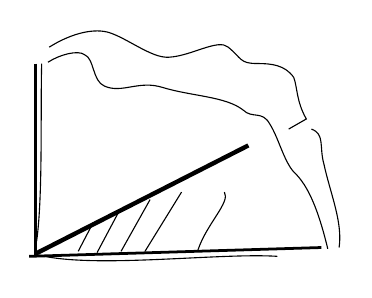
\begin{tikzpicture}[x=0.016cm,y=-0.016cm]
\draw[line width=1pt] (21,35)--(21,187);
\draw (26,35) .. controls (25,75) and (27,140) .. (22,176);
\draw[line width=1pt] (16,188)--(248,181);
\draw (24,187) .. controls (68,198) and (167,185) .. (213,188);
\draw (31,34) .. controls (40,28) and (55,24) .. (60,28)
.. controls (68,31) and (66,49) .. (76,53)
.. controls (90,59) and (103,48) .. (122,54)
.. controls (145,61) and (172,61) .. (186,72)
.. controls (193,79) and (201,72) .. (207,83)
.. controls (214,94) and (218,112) .. (226,121)
.. controls (238,132) and (246,153) .. (253,182);
\draw (32,22) .. controls (48,12) and (65,7) .. (78,10)
.. controls (93,14) and (113,31) .. (127,30)
.. controls (145,29) and (166,15) .. (174,22)
.. controls (185,31) and (183,35) .. (197,35)
.. controls (208,35) and (219,36) .. (226,46)
.. controls (229,54) and (228,65) .. (236,79)
--(222,87);
\draw (240,87) .. controls (251,91) and (246,101) .. (250,115)
.. controls (255,138) and (265,161) .. (262,181);
\draw[line width=1.6pt] (21,186)--(190,100);
\draw (55,184)--(67,161);
\draw (70,185)--(87,153);
\draw (89,184)--(112,143);
\draw (108,184)--(137,137);
\draw (150,183) .. controls (157,162) and (176,145) .. (171,137);
\end{tikzpicture}}

La \deleted{condition} \inserted{c)} \unsure{impliquent|implique} que si $j'$ est
un prédécesseur de $j$, et si $k\in I$ est $\le j$
mais non $\le j'$, et s'il existe
un $i$ majoré par $k$ et $j'$, \uline{alors}
$k'=\operatorname{Inf}(k,j')$ existe, et $k'$ est
un prédécesseur de $k$.

\diagram{\begin{tikzcd}[column sep=small,row sep=small]
& j' \arrow[r,leftrightarrow,"\mathrm{préd}"'] \arrow[d,phantom,"{\rotatebox{90}{$\leq$}}" description] & j \arrow[d,phantom,"{\rotatebox{90}{$\leq$}}" description] \\
& k' \arrow[r,leftrightarrow] & k \\
i \arrow[uur,hook] \arrow[urr,hook] & &
\end{tikzcd}}

(Il suffit de voir que dans
un ens. ordonné de la forme $\mathcal P(\unsure{\sigma|F})$,
les inf exist (c'est l'intersection) et si
$j'\subset j=j'\amalg\{\alpha\}$, et $k\in j$ mais non $k\subset j'$,
alors \deleted{$\unsure{k\ne k'}$} $k=k'\amalg\{\alpha\}$ avec $k'=k\cap j'$, ..)
\margin{$\sigma$ ens fini}

Ceci posé, considérons le diagramme
\diagram{\begin{tikzcd}
X_{j'} \arrow[r,hook] & X_j \\
X_{k'} \arrow[u] \arrow[r,hook] & X_k \arrow[u]
\end{tikzcd}}
où les flèches verticales, par l'hyp. $\unsure{1^\circ)|16)}$,
sont des plongements bordants. Ceci posé, on
voit \inserted{(par b,c)} que \deleted{$(X_k\longrightarrow X_{\unsure{j}}$.}
$(X_k,X_{k'})\mathbin{-}(X_j,X_{j'})$
\margin{28}
